% LaTeX file for resume 

% The value for margin is ignored, but it has to be there or geometry throws
% errors. The margin option causes section titles to appear to the left of body text 
\documentclass[margin]{res} 
\usepackage{graphicx}
\usepackage{anysize}
\usepackage{hyperref}
\marginsize{0.3in}{1.7in}{0.3in}{0.5in}
\renewcommand{\labelitemi}{\tiny \textbullet}

\begin{document} 

\name{\textsf{Russell E. Harmon}}

\address{\textsf{{\bf School Address}} \\ \textsf{Rochester Institute of Technology}
\\ \textsf{Computer Science} \\ \textsf{39 Nathaniel Rochester Hall} \\
\textsf{Rochester, NY 14623}}
\address{\textsf{{\bf Permanent Address}} \\ \textsf{2710 Avenue J N/W} \\
\textsf{Winter Haven, FL 33881} \\ \textsf{(863) 514-7014} \\
\textsf{russ@eatnumber1.com}}
 
\begin{resume}

\section{\textsf{Education}}
	\begin{itemize} \itemsep -2pt
		\item {\bf Rochester Institute of Technology} – Computer Science, minor
		in Music. \hfill {\footnotesize 2006 - Present}
		\item {\bf Herbert H. Lehman High School} - College Prep Program \hfill
		{\footnotesize 2002 - 2006}
		\begin{itemize} \itemsep -2pt
			\item {\small AP English}
		\end{itemize}
		\item {\bf Lehman College} - Course work in Q-Basic (age 12)
	\end{itemize}

\section{\textsf{Experience}}
	\begin{itemize} \itemsep -2pt
		\item {\bf SafeNet Inc}, Belcamp, MD \hfill {\small June 2008 - November
		2008}
		\\* Engineering Intern \hfill {\footnotesize http://www.safenet-inc.com}
		\begin{itemize} \itemsep -2pt
			\item {\small Work as a developer on a team of 7 on SMCII (the SafeNet
			Management Console).}
			\item {\small Java development with JBoss, Hibernate and JSF}
		\end{itemize}
		\item {\bf New York City Department of Education}, Bronx, NY \hfill
		{\small September 2002 - June 2006}
		\\* IT Specialist \hfill {\footnotesize http://schools.nyc.gov}
		\begin{itemize} \itemsep -2pt
			\item {\small Setup and maintain computer systems throughout Lehman
			High School}
			\item {\small Diagnose, repair, and maintain the network}
			\item {\small Reformat machines using Norton Ghost}
			\item {\small When the school got new machines, I had to migrate
			user's settings onto the new machines}
			\item {\small Diagnose and eliminate viruses and malware on the
			school's network and computer systems}
			\item {\small Audit the network for malicious activity}
		\end{itemize}

		\item {\bf New York Sailing \& Yacht Club}, Bronx, NY \hfill {\small
		2001-2005}
		\\* Launch Operator \hfill {\footnotesize http://www.startsailing.com}
		\begin{itemize} \itemsep -2pt
			\item {\small Taxi patrons to their boats moored in the harbor}
			\item {\small Experienced in both motor and sail powered small craft
			operation}
		\end{itemize}

		\item {\bf City Island Computer Services}, Bronx, NY \hfill {\small
		1998-1999}
		\\* Apprentice (age 10)
	\end{itemize}

\section{\textsf{Technical Skills}}
	\begin{itemize} \itemsep -2pt
		\item Cisco switches
		\item UNIX
		\begin{itemize} \itemsep -2pt
			\item {\small Linux}
			\item {\small Solaris}
			\item {\small BSD}
		\end{itemize}
		\item Java
		\item C
		\item C++
		\item Python
		\item PC troubleshooting and repair
	 \end{itemize}

\section{\textsf{Honors and Awards}}
	\begin{itemize} \itemsep -2pt
		\item NYC regional robotics award winner – 27th place in the national competition
		\item Honor roll 2003-2005
		\item Visual Basic Programming Award for academic excellence, 2005
		\item First Place Sailing Award 2000, 2002
	\end{itemize}

\section{\textsf{Special Accomplishments}}
	\begin{itemize} \itemsep -2pt
		\item At age 8 built my first computer, at age 12 attended my first programming class at Lehman College.
		\item Designed and implemented an encryption algorithm using a combination of transposition and substitution.
		\item Rocking the Boat – built a boat for needy children from the South Bronx.
	\end{itemize}

\section{\textsf{Certifications}}
	\begin{itemize} \itemsep -2pt
		\item Cisco Academy, with honors (terms 1 and 2)
		\item A+
		\item MOUS (Word)
	\end{itemize}

\end{resume}
\pagebreak[4] % The 4 makes it a VERY INSISTENT requirement for a page break.
\marginsize{-1.5in}{-1.5in}{-0.5in}{-0.5in}
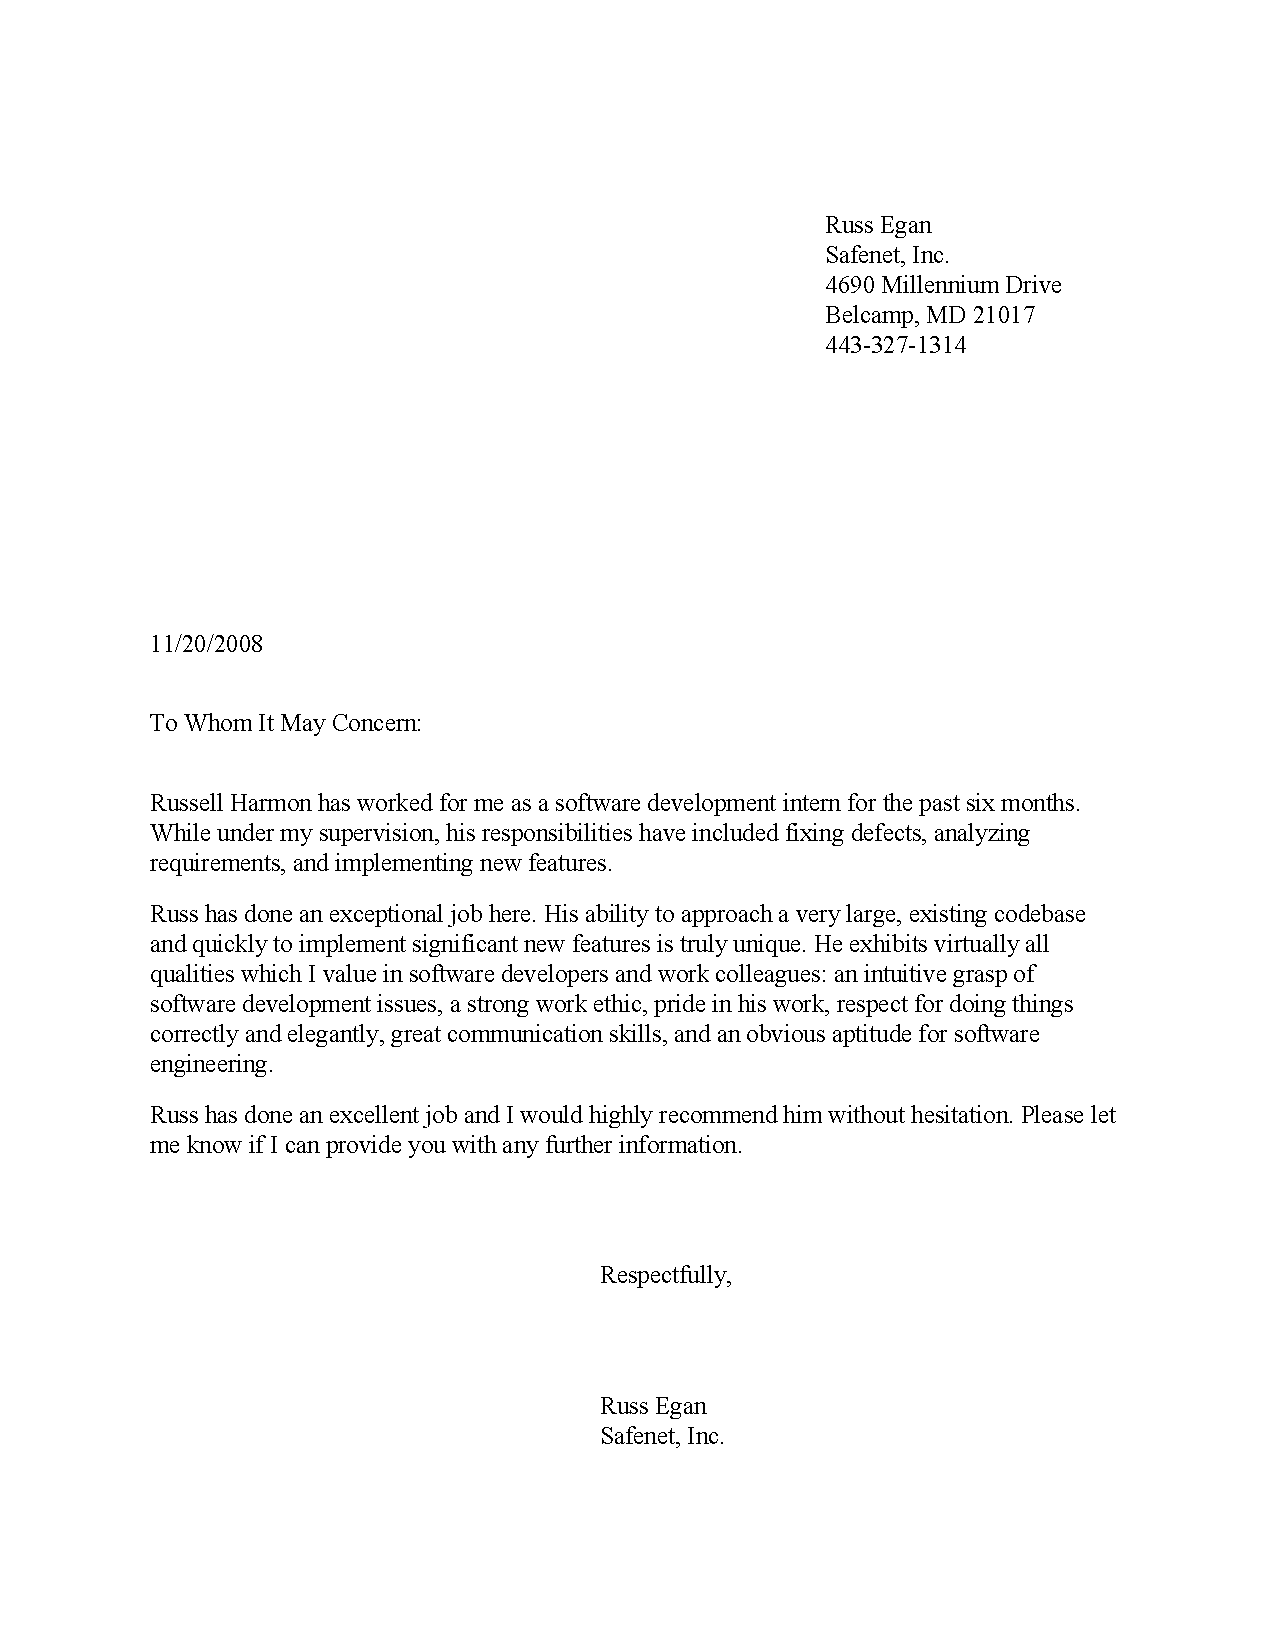
\includegraphics{sfnt-recommendation.pdf}
\end{document}
